\section{Alternative Explanation for Emergent Abilities}
\label{sec:alt_explanation}

\begin{figure}
    \centering
    % 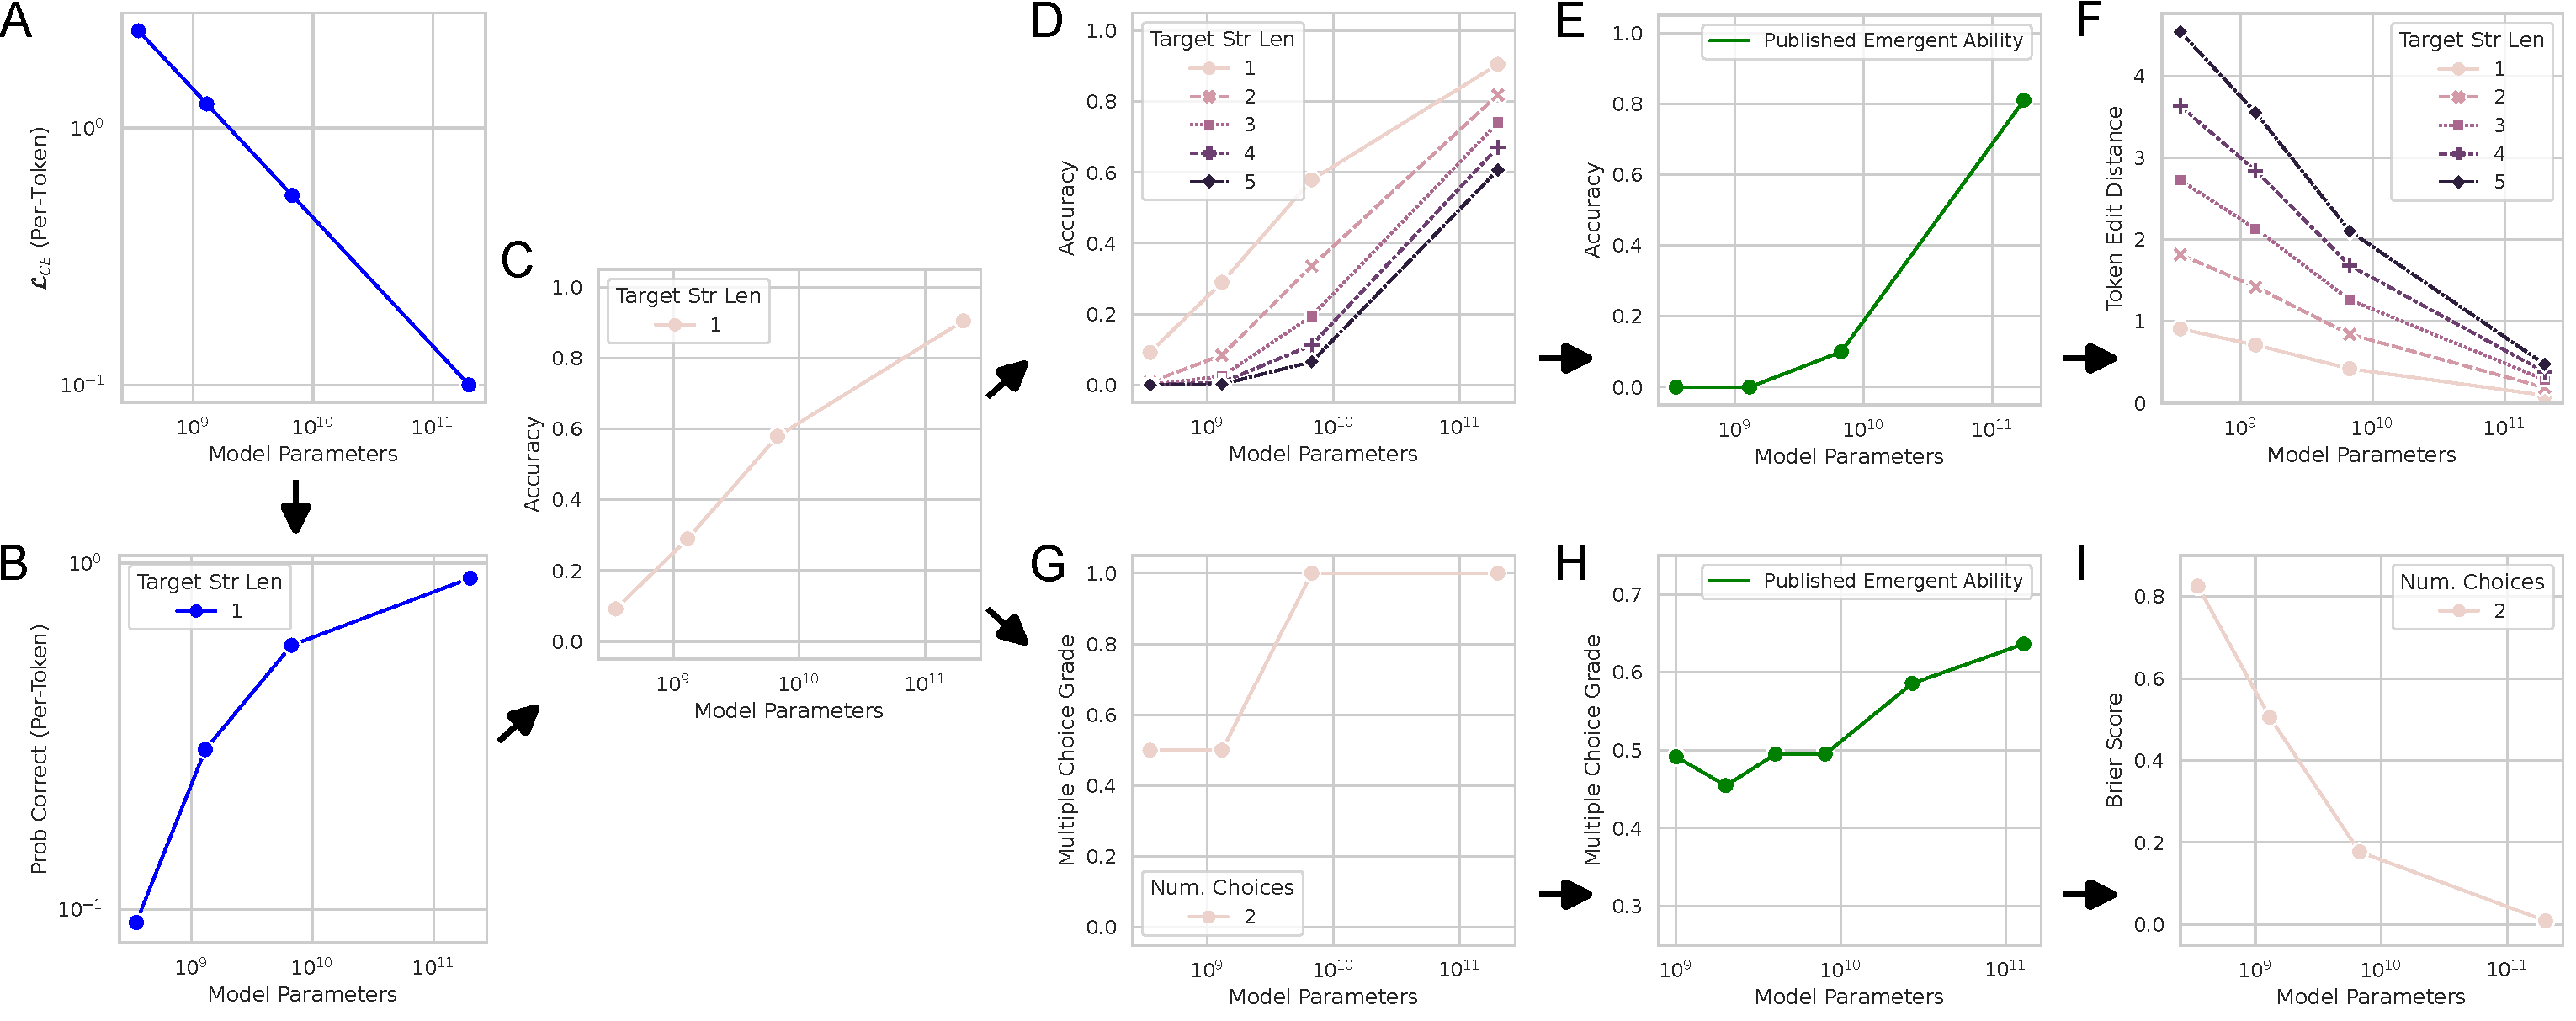
\includegraphics[width=\textwidth]{figures/toy_emergence/toy_analytical_model.pdf}
    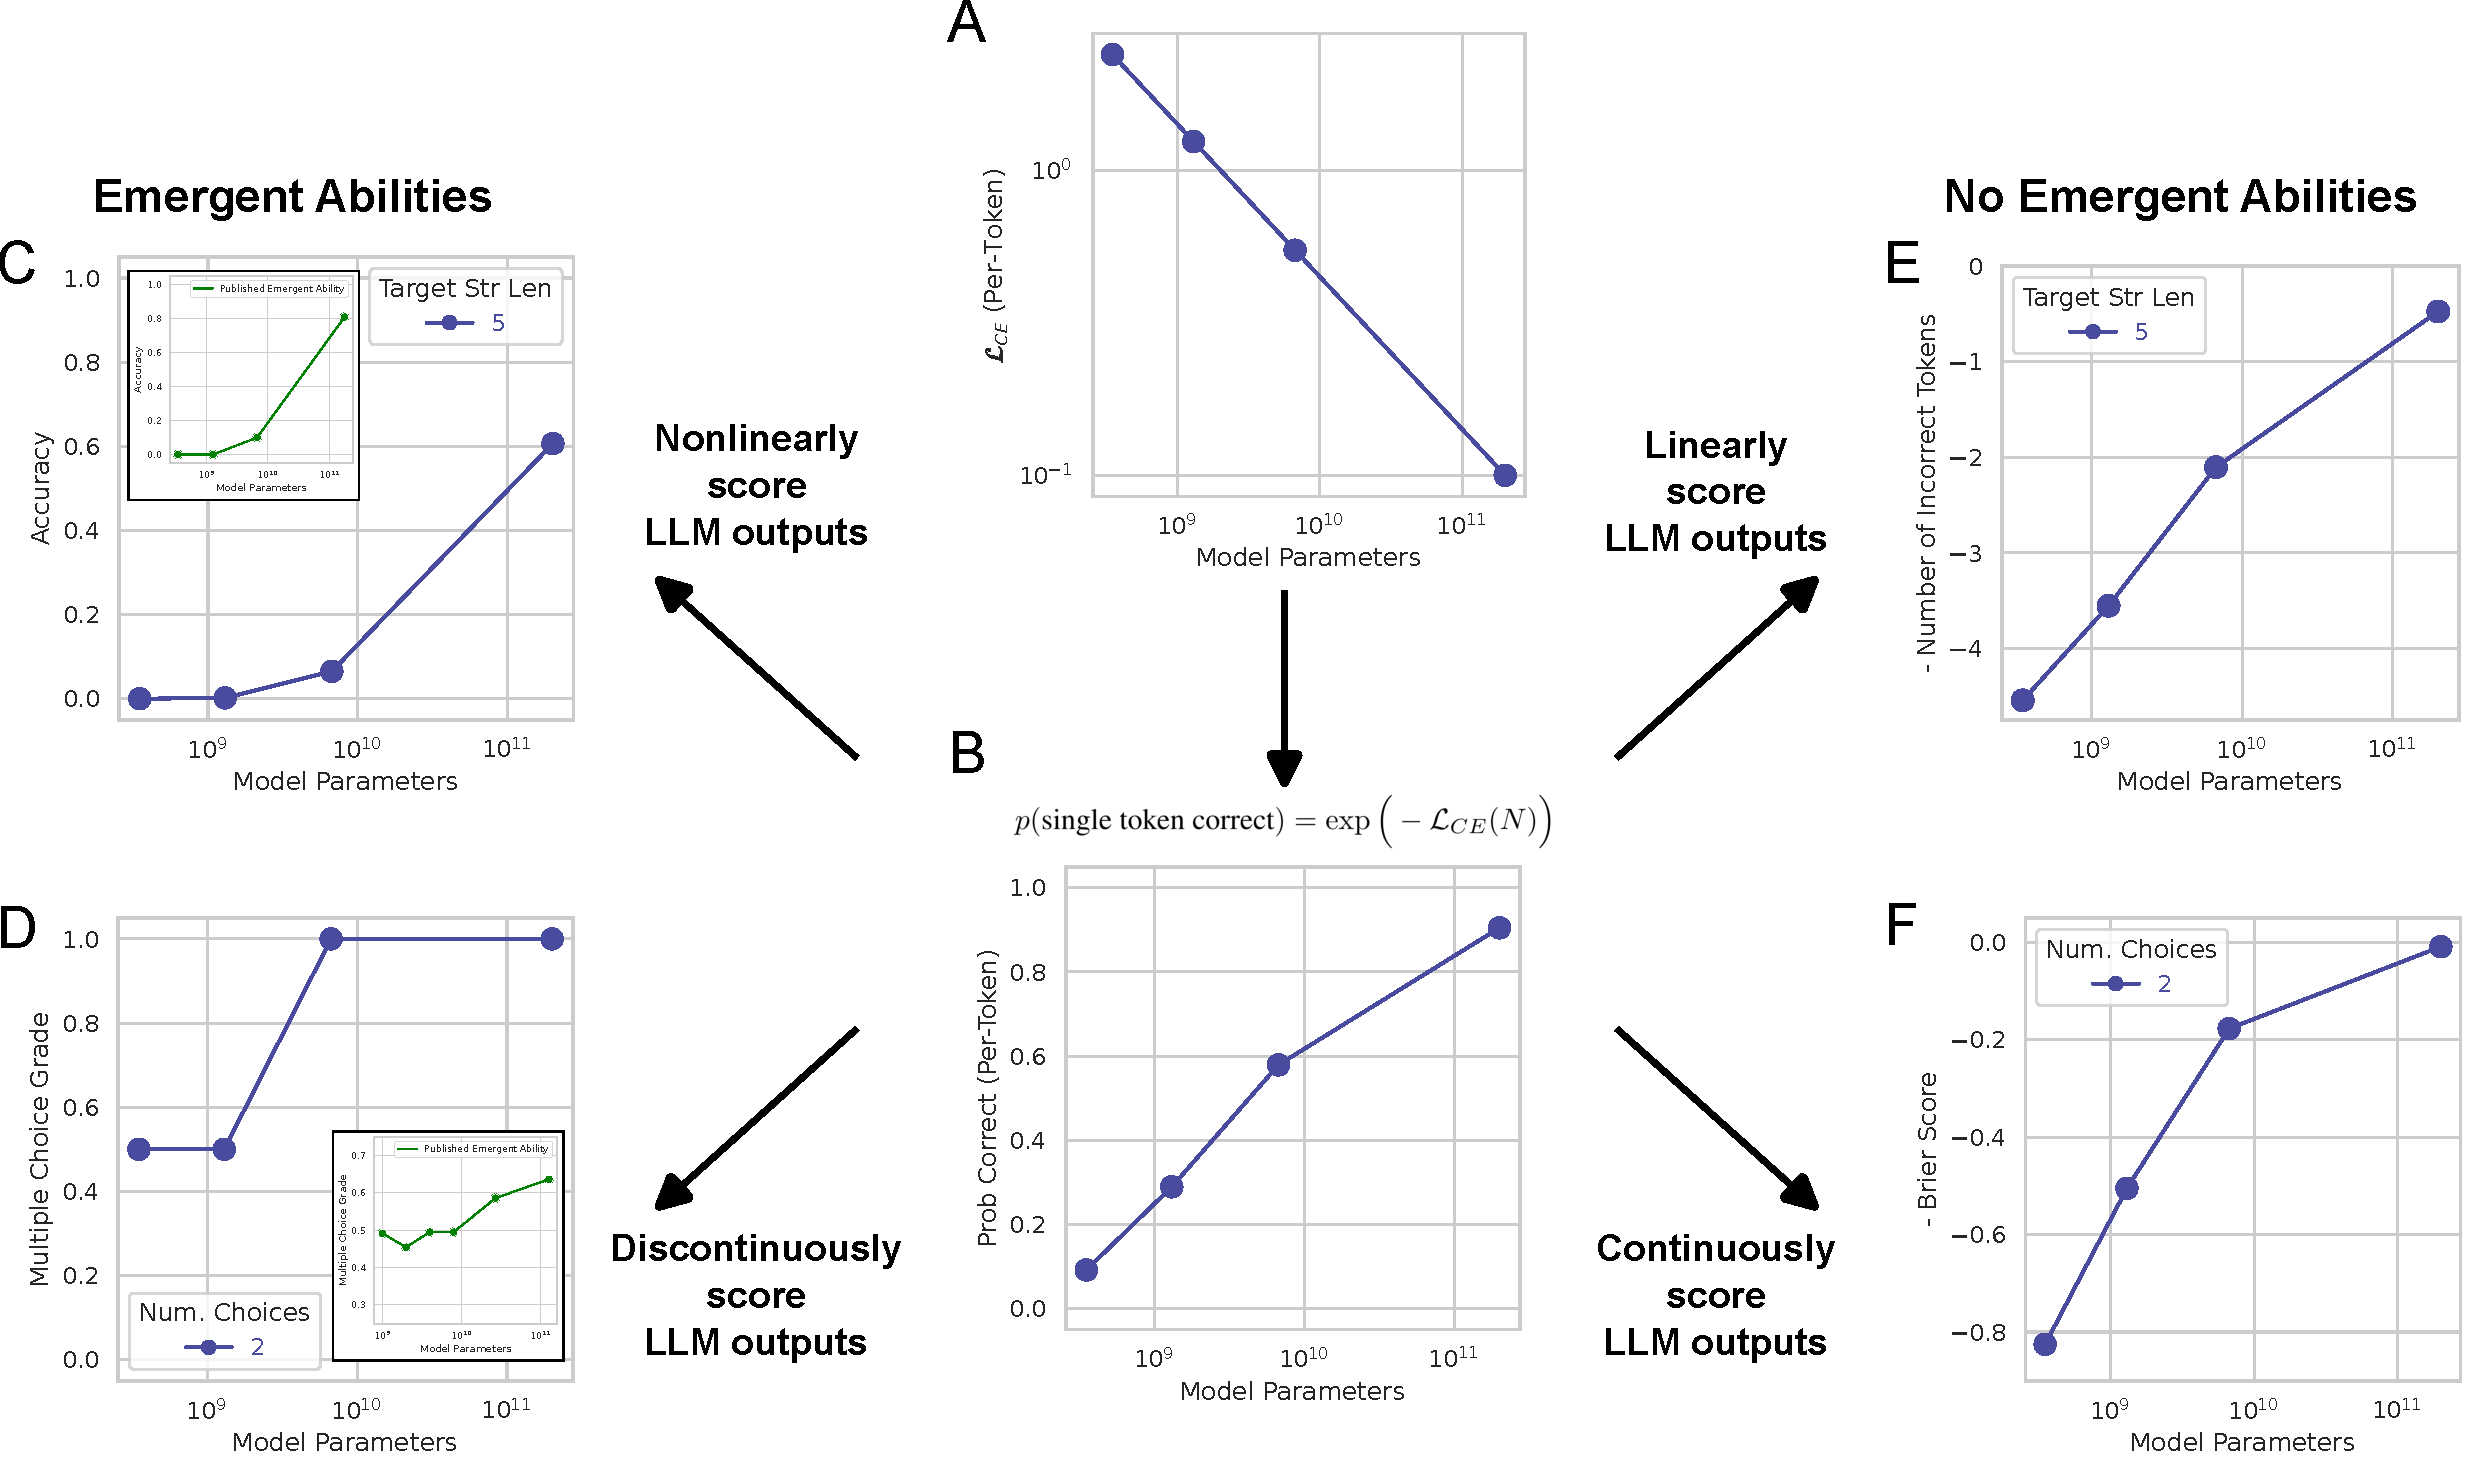
\includegraphics[width=0.9\textwidth]{figures/toy_emergence/toy_analytical_model_try2.pdf}
    \caption{\textbf{Emergent abilities of large language models are created by the researcher's chosen metrics, not unpredictable changes in model behavior with scale.} (A) Suppose the per-token cross-entropy loss decreases monotonically with model scale, e.g., $\mathcal{L}_{CE}$ scales as a power law. (B) The per-token probability of selecting the correct token asymptotes towards 1. (C) If the researcher scores models' outputs using a nonlinear metric such as Accuracy (which requires a sequence of tokens to \textit{all} be correct), the metric choice nonlinearly scales performance, causing performance to change sharply and unpredictably in a manner that qualitatively matches published emergent abilities (inset). (D) If the researcher instead scores models' outputs using a discontinuous metric such as Multiple Choice Grade (akin to a step function), the metric choice discontinuously scales performance, again causing performance to change sharply and unpredictably. (E) Changing from a nonlinear metric to a linear metric such as Token Edit Distance, scaling shows smooth, continuous and predictable improvements, ablating the emergent ability. (F) Changing from a discontinuous metric to a continuous metric such as Brier Score again reveals smooth, continuous and predictable improvements in task performance. Consequently, emergent abilities are created by the researcher's choice of metrics, not fundamental changes in model family behavior on specific tasks with scale.}
    \label{fig:toy_model}
\end{figure}

How might smooth, continuous, predictable changes in model family performance appear sharp and unpredictable?
% The answer is that even if the per-token error rate changes smoothly with scale, the researcher's choice of a nonlinear or discontinuous metric can distort the model family's performance to appear sharp and unpredictable.
The answer is that the researcher's choice of a nonlinear or discontinuous metric can distort the model family's performance to appear sharp and unpredictable.

To expound, suppose that within a model family, the test loss falls smoothly, continuously and predictably with the number of model parameters.
One reason to believe this is the phenomenon known as neural scaling laws: empirical observations that deep networks exhibit power law scaling in the test loss as a function of training dataset size, number of parameters or compute \citep{hestness2017deep,rosenfeld2019constructive,henighan2020scaling,kaplan2020scaling,gordon2021data,hernandez2021scaling,jones2021scaling,zhai2022scaling,hoffmann2022training, clark2022unified, neumann2022scaling}.
%this finding has been observed spanning 7 orders of magnitude across diverse domains including vision and language modeling.
%Motivated by neural scaling laws, 
For concreteness, suppose we have a model family of different numbers of parameters $N > 0$ and assume that each model's per-token cross entropy falls as a power law with the number of parameters $N$ for constants $c > 0, \alpha < 0$ (Fig. \ref{fig:toy_model}A):

\begin{equation*}
    \mathcal{L}_{CE}(N) = \Big(\frac{N}{c}\Big)^{\alpha}
\end{equation*}

To be clear, we do not require this particular functional form to hold; rather, we use it for illustrative purposes.
Let $V$ denote the set of possible tokens, $p \in \Delta^{|V|-1}$ denote the true but unknown probability distribution, and $\hat{p}_N \in \Delta^{|V|-1}$ denote the $N$-parameter model's predicted probability distribution.
The per-token cross entropy as a function of number of parameters $N$ is:

\begin{equation*}
    \mathcal{L}_{CE}(N) \; \defeq \; - \sum_{v \in V} p(v) \log \hat{p}_N(v)
\end{equation*}

In practice, $p$ is unknown, so we substitute a one-hot distribution of the observed token $v^*$:

\begin{equation*}
    \mathcal{L}_{CE}(N) = - \log \hat{p}_N(v^*)
\end{equation*}

A model with $N$ parameters then has a per-token probability of selecting the correct token (Fig. \ref{fig:toy_model}B):

\begin{equation*}
    p(\text{single token correct}) = \exp \Big(- \mathcal{L}_{CE}(N) \Big) =\exp \Big(- (N/c)^{\alpha} \Big)
\end{equation*}

%As a  sanity check, note that as the number of parameters increases (decreases), the per-token accuracy asymptotes towards 1 (towards 0).
Suppose the researcher then chooses a metric that requires selecting $L$ tokens correctly.
For example, our task might be $L$-digit integer addition, and a model's output is scored $1$ if all $L$ output digits exactly match all target digits with no additions, deletions or substitutions, $0$ otherwise.
If the probability each token is correct is independent\footnote{While the independence assumption is not true, the approximation yields results qualitatively matching the observed emergence claims.}, the probability of scoring $1$ is:

\begin{equation*}
    \text{Accuracy}(N) \approx p_N(\text{single token correct})^{\text{num. of tokens}} = \exp \Big(- (N/c)^{\alpha} \Big)^L
\end{equation*}

This choice of metric nonlinearly scales performance with increasing token sequence length. When plotting performance on a linear-log plot, one sees a sharp, unpredictable emergent ability on longer sequences  (Fig. \ref{fig:toy_model}C) that closely matches claimed emergent abilities (inset).
What happens if the researcher switches from a nonlinear metric like Accuracy, under which the per-token error rate scales geometrically in target length (App. \ref{app:metric_scaling:accuracy}), to an approximately linear metric like Token Edit Distance, under which the per-token error rate scales quasi-linearly in target length (App. \ref{app:metric_scaling:token_edit_distance})?

\begin{equation*}
    \text{Token Edit Distance}(N) \approx L \, \Big(1 - p_N(\text{single token correct}) \Big) = L \, \Big( 1 - \exp \big(- (N/c)^{\alpha} \big) \Big)
\end{equation*}

The linear metric reveals smooth, continuous, predictable changes in model performance (Fig. \ref{fig:toy_model}E).
Similarly, if the researcher uses a discontinuous metric like Multiple Choice Grade, the researcher can find emergent abilities (Fig. \ref{fig:toy_model}D), but switching to a continuous metric like Brier Score removes the emergent ability (Fig. \ref{fig:toy_model}F).
In summary, sharp and unpredictable changes with increasing scale can be fully explained by three interpretable factors: (1) the researcher choosing a metric that nonlinearly or discontinuously scales the per-token error rate, (2) having insufficient resolution to estimate model performance in the smaller parameter regime, with resolution\footnote{Resolution is defined as ``The smallest interval measurable by a scientific instrument; the resolving power."} set by $1/\text{test dataset size}$, and (3) insufficiently sampling the larger parameter regime. 